\documentclass[letterpaper,12pt]{article}\usepackage[]{graphicx}\usepackage[]{color}
%% maxwidth is the original width if it is less than linewidth
%% otherwise use linewidth (to make sure the graphics do not exceed the margin)
\makeatletter
\def\maxwidth{ %
  \ifdim\Gin@nat@width>\linewidth
    \linewidth
  \else
    \Gin@nat@width
  \fi
}
\makeatother

\definecolor{fgcolor}{rgb}{0.345, 0.345, 0.345}
\newcommand{\hlnum}[1]{\textcolor[rgb]{0.686,0.059,0.569}{#1}}%
\newcommand{\hlstr}[1]{\textcolor[rgb]{0.192,0.494,0.8}{#1}}%
\newcommand{\hlcom}[1]{\textcolor[rgb]{0.678,0.584,0.686}{\textit{#1}}}%
\newcommand{\hlopt}[1]{\textcolor[rgb]{0,0,0}{#1}}%
\newcommand{\hlstd}[1]{\textcolor[rgb]{0.345,0.345,0.345}{#1}}%
\newcommand{\hlkwa}[1]{\textcolor[rgb]{0.161,0.373,0.58}{\textbf{#1}}}%
\newcommand{\hlkwb}[1]{\textcolor[rgb]{0.69,0.353,0.396}{#1}}%
\newcommand{\hlkwc}[1]{\textcolor[rgb]{0.333,0.667,0.333}{#1}}%
\newcommand{\hlkwd}[1]{\textcolor[rgb]{0.737,0.353,0.396}{\textbf{#1}}}%

\usepackage{framed}
\makeatletter
\newenvironment{kframe}{%
 \def\at@end@of@kframe{}%
 \ifinner\ifhmode%
  \def\at@end@of@kframe{\end{minipage}}%
  \begin{minipage}{\columnwidth}%
 \fi\fi%
 \def\FrameCommand##1{\hskip\@totalleftmargin \hskip-\fboxsep
 \colorbox{shadecolor}{##1}\hskip-\fboxsep
     % There is no \\@totalrightmargin, so:
     \hskip-\linewidth \hskip-\@totalleftmargin \hskip\columnwidth}%
 \MakeFramed {\advance\hsize-\width
   \@totalleftmargin\z@ \linewidth\hsize
   \@setminipage}}%
 {\par\unskip\endMakeFramed%
 \at@end@of@kframe}
\makeatother

\definecolor{shadecolor}{rgb}{.97, .97, .97}
\definecolor{messagecolor}{rgb}{0, 0, 0}
\definecolor{warningcolor}{rgb}{1, 0, 1}
\definecolor{errorcolor}{rgb}{1, 0, 0}
\newenvironment{knitrout}{}{} % an empty environment to be redefined in TeX

\usepackage{alltt}
\usepackage[top=1in,bottom=1in,left=1in,right=1in]{geometry}
\usepackage{setspace}
\usepackage[colorlinks=true,urlcolor=blue,citecolor=blue,linkcolor=blue]{hyperref}
\usepackage{indentfirst}
\usepackage{multirow}
\usepackage{booktabs}
\usepackage[final]{animate}
\usepackage{graphicx}
\usepackage{verbatim}
\usepackage{rotating}
\usepackage{tabularx}
\usepackage{array}
\usepackage{subfig} 
\usepackage[noae]{Sweave}
\usepackage{cleveref}
\usepackage[figureposition=bottom]{caption}
\usepackage{paralist}
\usepackage{acronym}
\usepackage{outlines}
\usepackage{pdflscape}

% knitr options


\IfFileExists{upquote.sty}{\usepackage{upquote}}{}
\begin{document}

\setlength{\parskip}{5mm}
\setlength{\parindent}{0in}

\title{Summary of data processing for Patuxent River Estuary}
\author{Marcus W. Beck, Rebecca Murphy}
\maketitle

The following describes additional processing of raw station data for the Patuxent River Estuary. Note that the raw data file (`PAX\_TRIB...') was edited manually to remove station TF1.0 and to change the chlorophyll value for TF1.4 on 11/28/1988 from 2.99 to 5.98.  All data for 1985 was also removed because of incomplete coverage for many stations.  Brief descriptions of additional processing steps are provided below.

The following raw data files were imported:
\begin{enumerate}
\item \texttt{PAX\_TRIB\_CHLAandSALINITY\_85to14.csv}: chlorophyll and salinity data for all stations in the Patuxent River from 1985 to 2014 (from R. Murphy)
\item \texttt{PAX\_station\_info.csv}: metadata for each station including lat/lon, salinity zone, etc. (from R. Murphy) - not used in this document
\end{enumerate}

The data were first imported into R.
\begin{kframe}
\begin{alltt}
\hlcom{# code for processing raw data, see email from R. Murphy on 3/13/15}
\hlcom{# created March 2015, M. Beck}

\hlcom{## packages to use}
\hlcom{# this is just to load dplyr, ggplot2}
\hlstd{devtools}\hlopt{::}\hlkwd{load_all}\hlstd{(}\hlstr{'M:/docs/tidal_comp/TidalComp'}\hlstd{)}

\hlcom{## import}

\hlcom{# meta}
\hlstd{pax_meta} \hlkwb{<-} \hlkwd{system.file}\hlstd{(}\hlstr{'PAX_station_info.csv'}\hlstd{,} \hlkwc{package} \hlstd{=} \hlstr{'TidalComp'}\hlstd{)}
\hlstd{pax_meta} \hlkwb{<-} \hlkwd{read.csv}\hlstd{(pax_meta,} \hlkwc{header} \hlstd{=} \hlnum{TRUE}\hlstd{,}
  \hlkwc{stringsAsFactors} \hlstd{=} \hlnum{FALSE}\hlstd{)}

\hlcom{# data}
\hlstd{pax_data} \hlkwb{<-} \hlkwd{system.file}\hlstd{(}\hlstr{'PAX_TRIB_CHLAandSALINITY_85TO14.csv'}\hlstd{,}
  \hlkwc{package} \hlstd{=} \hlstr{'TidalComp'}\hlstd{)}
\hlstd{pax_data} \hlkwb{<-} \hlkwd{read.csv}\hlstd{(pax_data,} \hlkwc{header} \hlstd{=} \hlnum{TRUE}\hlstd{,}
  \hlkwc{stringsAsFactors} \hlstd{=} \hlnum{FALSE}\hlstd{)}

\hlcom{# remove 1985 from pax_data}
\hlstd{pax_data} \hlkwb{<-} \hlkwd{filter}\hlstd{(pax_data,} \hlopt{!}\hlkwd{grepl}\hlstd{(}\hlstr{'/1985$'}\hlstd{, date))}

\hlcom{# reorder STATION variable along trib axis}
\hlstd{stats} \hlkwb{<-} \hlkwd{c}\hlstd{(}\hlstr{'TF1.3'}\hlstd{,} \hlstr{'TF1.4'}\hlstd{,} \hlstr{'TF1.5'}\hlstd{,} \hlstr{'TF1.6'}\hlstd{,} \hlstr{'TF1.7'}\hlstd{,}
  \hlstr{'RET1.1'}\hlstd{,} \hlstr{'LE1.1'}\hlstd{,} \hlstr{'LE1.2'}\hlstd{,} \hlstr{'LE1.3'}\hlstd{,} \hlstr{'LE1.4'}\hlstd{)}
\hlstd{pax_data}\hlopt{$}\hlstd{STATION} \hlkwb{<-} \hlkwd{factor}\hlstd{(pax_data}\hlopt{$}\hlstd{STATION,} \hlkwc{level} \hlstd{= stats)}
\end{alltt}
\end{kframe}

Salinity data were vertically-integrated for each  unique date. The integration function averaged all salinity values after interpolating from the surface to the maximum depth.  Salinity values at the most shallow and deepest sampling depth were repeated for zero depth and maximum depths, respectively, to bound the interpolations within the range of the data.
\begin{kframe}
\begin{alltt}
\hlcom{##}
\hlcom{# get vertically integrated salinity}

\hlcom{# function for vertical integration}
\hlstd{int_fun} \hlkwb{<-} \hlkwa{function}\hlstd{(}\hlkwc{TOTAL_DEPTH}\hlstd{,} \hlkwc{DEPTH}\hlstd{,} \hlkwc{AvgValue}\hlstd{)\{}

  \hlcom{# only interpolate if > 1 salinity value}
  \hlkwa{if}\hlstd{(}\hlkwd{length}\hlstd{(}\hlkwd{na.omit}\hlstd{(AvgValue))} \hlopt{<} \hlnum{2} \hlstd{)} \hlkwd{return}\hlstd{(}\hlkwd{na.omit}\hlstd{(AvgValue))}

  \hlcom{# setup for interpolation}
  \hlstd{max_depths} \hlkwb{<-} \hlkwd{mean}\hlstd{(}\hlkwd{unique}\hlstd{(TOTAL_DEPTH),} \hlkwc{na.rm} \hlstd{=} \hlnum{TRUE}\hlstd{)}
  \hlstd{depths} \hlkwb{<-} \hlkwd{c}\hlstd{(}\hlnum{0}\hlstd{, DEPTH, max_depths)}
  \hlstd{vals} \hlkwb{<-} \hlkwd{c}\hlstd{(AvgValue[}\hlnum{1}\hlstd{], AvgValue, AvgValue[}\hlkwd{length}\hlstd{(AvgValue)])}

  \hlcom{# get the average of the interpolation}
  \hlstd{out} \hlkwb{<-} \hlkwd{mean}\hlstd{(}\hlkwd{approx}\hlstd{(depths, vals)}\hlopt{$}\hlstd{y)}

  \hlkwd{return}\hlstd{(out)}

  \hlstd{\}}

\hlcom{# process}
\hlcom{# note that there are no 'PROBLEM' values, lab and method do not change}
\hlstd{sal_tmp} \hlkwb{<-} \hlkwd{filter}\hlstd{(pax_data, PARAMETER} \hlopt{==} \hlstr{'SALINITY'}\hlstd{)} \hlopt
  \hlkwd{mutate}\hlstd{(}\hlkwc{date} \hlstd{=} \hlkwd{as.Date}\hlstd{(date,} \hlkwc{format} \hlstd{=} \hlstr{'%m/%d/%Y'}\hlstd{))} \hlopt
  \hlkwd{group_by}\hlstd{(date, STATION)} \hlopt
  \hlkwd{summarize}\hlstd{(}\hlkwc{sal} \hlstd{=} \hlkwd{int_fun}\hlstd{(TOTAL_DEPTH, DEPTH, AvgValue))}
\end{alltt}
\end{kframe}

Chlorophyll values at each station were retained only for surface samples and no `problem' codes.  Chlorophyll were also transformed with the natural-log.  
\begin{kframe}
\begin{alltt}
\hlcom{##}
\hlcom{# get only surface estimates for chlorophyll}
\hlcom{# remove those w/ problem codes (only a few obs)}
\hlstd{chl_tmp} \hlkwb{<-} \hlkwd{filter}\hlstd{(pax_data,}
  \hlstd{PARAMETER} \hlopt{==} \hlstr{'CHLA'} \hlopt{&} \hlstd{LAYER} \hlopt{==} \hlstr{'S'}\hlopt{&} \hlstd{PROBLEM} \hlopt{==} \hlstr{''}
  \hlstd{)} \hlopt
  \hlkwd{mutate}\hlstd{(}\hlkwc{lnchla} \hlstd{=} \hlkwd{log}\hlstd{(AvgValue))} \hlopt
  \hlkwd{mutate}\hlstd{(}\hlkwc{date} \hlstd{=} \hlkwd{as.Date}\hlstd{(date,} \hlkwc{format} \hlstd{=} \hlstr{'%m/%d/%Y'}\hlstd{))} \hlopt
  \hlkwd{select}\hlstd{(date, STATION, lnchla)}
\end{alltt}
\end{kframe}

The data were recombined by date and station.  Some plots of the raw data are below.
\begin{kframe}
\begin{alltt}
\hlcom{## }
\hlcom{# merge chl and salinity data, then plot}

\hlstd{pax_data} \hlkwb{<-} \hlkwd{full_join}\hlstd{(chl_tmp, sal_tmp,} \hlkwc{by} \hlstd{=} \hlkwd{c}\hlstd{(}\hlstr{'date'}\hlstd{,} \hlstr{'STATION'}\hlstd{))}

\hlkwd{ggplot}\hlstd{(pax_data,} \hlkwd{aes}\hlstd{(}\hlkwc{x} \hlstd{= date,} \hlkwc{y} \hlstd{= sal,} \hlkwc{group} \hlstd{= STATION))} \hlopt{+}
  \hlkwd{geom_line}\hlstd{()} \hlopt{+}
  \hlkwd{theme_classic}\hlstd{()} \hlopt{+}
  \hlkwd{facet_wrap}\hlstd{(}\hlopt{~} \hlstd{STATION,} \hlkwc{ncol} \hlstd{=} \hlnum{3}\hlstd{)}

\hlkwd{ggplot}\hlstd{(pax_data,} \hlkwd{aes}\hlstd{(}\hlkwc{x} \hlstd{= date,} \hlkwc{y} \hlstd{= lnchla,} \hlkwc{group} \hlstd{= STATION))} \hlopt{+}
  \hlkwd{geom_line}\hlstd{()} \hlopt{+}
  \hlkwd{theme_classic}\hlstd{()} \hlopt{+}
  \hlkwd{facet_wrap}\hlstd{(}\hlopt{~} \hlstd{STATION,} \hlkwc{ncol} \hlstd{=} \hlnum{3}\hlstd{)}

\hlcom{# save the data}
\hlstd{save_path} \hlkwb{<-} \hlkwd{gsub}\hlstd{(}\hlstr{'text$'}\hlstd{,} \hlstr{'data'}\hlstd{,} \hlkwd{getwd}\hlstd{())}
\hlkwd{save}\hlstd{(pax_data,} \hlkwc{file} \hlstd{=} \hlkwd{paste0}\hlstd{(save_path,} \hlstr{'/pax_data.RData'}\hlstd{))}
\hlkwd{save}\hlstd{(pax_meta,} \hlkwc{file} \hlstd{=} \hlkwd{paste0}\hlstd{(save_path,} \hlstr{'/pax_meta.RData'}\hlstd{))}
\hlstd{save_path} \hlkwb{<-} \hlkwd{gsub}\hlstd{(}\hlstr{'text$'}\hlstd{,} \hlstr{'inst'}\hlstd{,} \hlkwd{getwd}\hlstd{())}
\hlkwd{write.csv}\hlstd{(pax_data,} \hlkwd{paste0}\hlstd{(save_path,} \hlstr{'/pax_data.csv'}\hlstd{),}
  \hlkwc{row.names} \hlstd{=} \hlnum{FALSE}\hlstd{,} \hlkwc{quote} \hlstd{=} \hlnum{FALSE}\hlstd{)}
\end{alltt}
\end{kframe}

{\centering 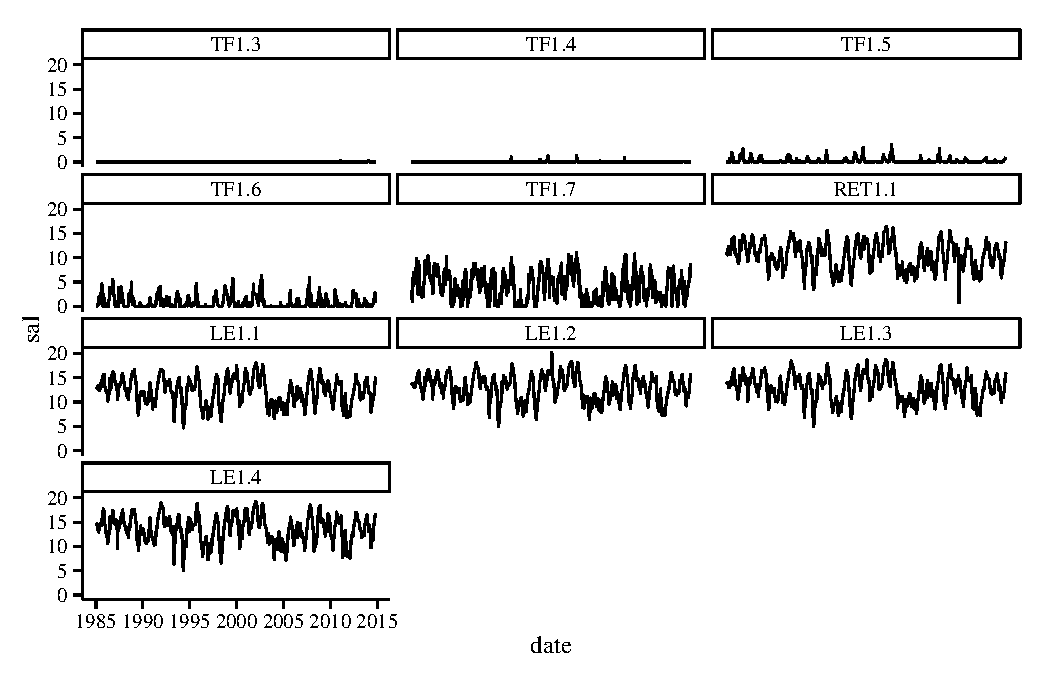
\includegraphics[width=\maxwidth]{figs/unnamed-chunk-41} 
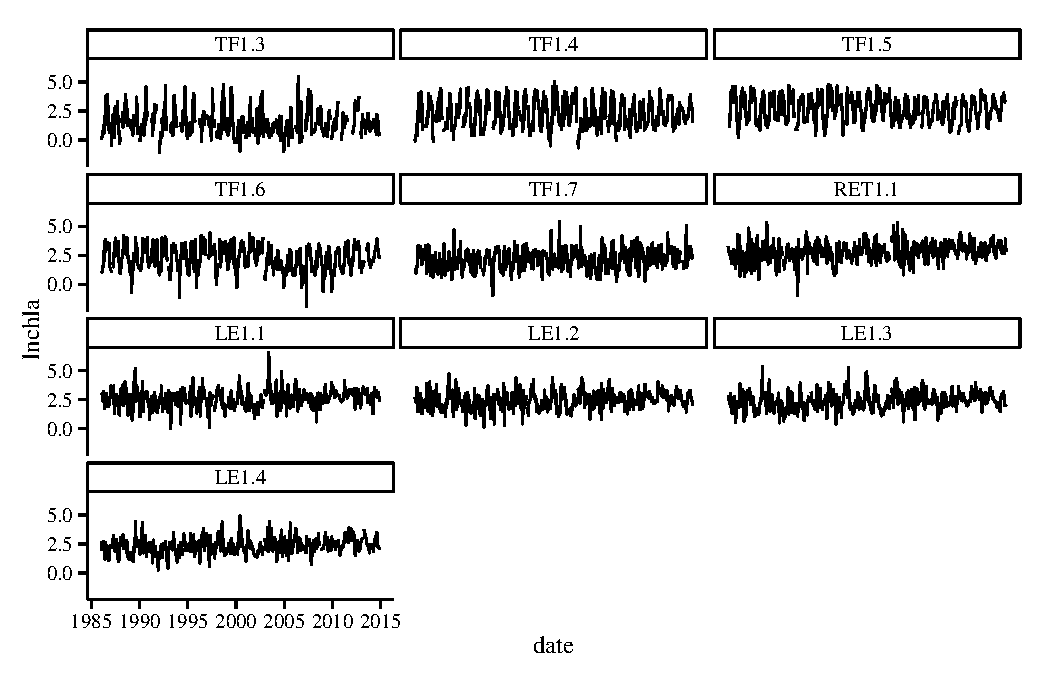
\includegraphics[width=\maxwidth]{figs/unnamed-chunk-42} 

}




Here are some more figures.

\begin{kframe}
\begin{alltt}
\hlstd{devtools}\hlopt{::}\hlkwd{load_all}\hlstd{()}
\hlkwd{data}\hlstd{(pax_data)}
\hlkwd{data}\hlstd{(pax_meta)}
\hlkwd{data}\hlstd{(pax_clip)}

\hlcom{# color palette}
\hlstd{cols} \hlkwb{<-} \hlkwd{wes_palette}\hlstd{(}\hlstr{'Zissou'}\hlstd{,} \hlnum{100}\hlstd{,} \hlstr{'continuous'}\hlstd{)} \hlopt
  \hlstd{as.character} \hlopt
  \hlstd{.[}\hlnum{1}\hlopt{:}\hlnum{60}\hlstd{]}

\hlcom{# change default ggplot theme}
\hlstd{theme_mine} \hlkwb{<-} \hlkwa{function} \hlstd{(}\hlkwc{base_size} \hlstd{=} \hlnum{12}\hlstd{,} \hlkwc{base_family} \hlstd{=} \hlstr{""}\hlstd{) \{}
  \hlkwd{theme_bw}\hlstd{(}\hlkwc{base_size} \hlstd{= base_size,} \hlkwc{base_family} \hlstd{= base_family)} \hlopt
  \hlkwd{theme}\hlstd{(}
    \hlkwc{axis.text.x} \hlstd{=} \hlkwd{element_text}\hlstd{(}\hlkwc{size} \hlstd{=} \hlnum{8}\hlstd{),}
    \hlkwc{plot.background} \hlstd{=} \hlkwd{element_rect}\hlstd{(}\hlkwc{fill}\hlstd{=}\hlstr{'transparent'}\hlstd{,}
      \hlkwc{colour} \hlstd{=} \hlnum{NA}\hlstd{),}
    \hlkwc{panel.background} \hlstd{=} \hlkwd{element_rect}\hlstd{(}\hlkwc{fill}\hlstd{=}\hlstr{'transparent'}\hlstd{,}
      \hlkwc{colour} \hlstd{=} \hlnum{NA}\hlstd{),}
    \hlkwc{legend.background} \hlstd{=} \hlkwd{element_rect}\hlstd{(}\hlkwc{fill}\hlstd{=}\hlstr{'transparent'}\hlstd{,}
      \hlkwc{colour} \hlstd{=} \hlnum{NA}\hlstd{),}
    \hlkwc{strip.background} \hlstd{=} \hlkwd{element_rect}\hlstd{(}\hlkwc{fill} \hlstd{=}
        \hlkwd{alpha}\hlstd{(cols[}\hlkwd{length}\hlstd{(cols)],} \hlnum{0.5}\hlstd{)),}
    \hlkwc{legend.key} \hlstd{=} \hlkwd{element_rect}\hlstd{(}\hlkwc{fill} \hlstd{=} \hlstr{'transparent'}\hlstd{,}
      \hlkwc{colour} \hlstd{=} \hlnum{NA}\hlstd{)}
    \hlstd{)}
\hlstd{\}}
\hlkwd{theme_set}\hlstd{(}\hlkwd{theme_mine}\hlstd{())}

\hlcom{# upper limit on boxplots}
\hlstd{y_max}\hlkwb{<-} \hlnum{7}
\hlstd{y_lab} \hlkwb{<-} \hlkwd{expression}\hlstd{(}
  \hlkwd{paste}\hlstd{(}\hlstr{'ln-chlorophyll  '}\hlstd{,}\hlkwd{italic}\hlstd{(a),}\hlstr{' ('}\hlstd{,}\hlkwd{italic}\hlstd{(mu),}\hlstr{'g'}\hlstd{,l}\hlopt{^-}\hlnum{1}\hlstd{,}\hlstr{')'}\hlstd{)}
  \hlstd{)}

\hlcom{# make plots for each station}
\hlstd{stats} \hlkwb{<-} \hlkwd{unique}\hlstd{(pax_meta}\hlopt{$}\hlstd{STATION)}
\hlkwd{pdf}\hlstd{(}\hlstr{'figs/pax_chl.pdf'}\hlstd{,} \hlkwc{height} \hlstd{=} \hlnum{5}\hlstd{,} \hlkwc{width} \hlstd{=} \hlnum{10}\hlstd{,} \hlkwc{family} \hlstd{=} \hlstr{'serif'}\hlstd{)}
\hlkwa{for}\hlstd{(stat} \hlkwa{in} \hlstd{stats)\{}

  \hlcom{# add yr, month columns}
  \hlstd{pax_stat} \hlkwb{<-} \hlkwd{filter}\hlstd{(pax_data, STATION} \hlopt{==} \hlstd{stat)} \hlopt
    \hlkwd{mutate}\hlstd{(}
      \hlkwc{mo} \hlstd{=} \hlkwd{strftime}\hlstd{(date,} \hlstr{'%m'}\hlstd{),}
      \hlkwc{yr} \hlstd{=} \hlkwd{strftime}\hlstd{(date,} \hlstr{'%Y'}\hlstd{)}
    \hlstd{)}

  \hlcom{# medians for plotting}
  \hlstd{yr_med} \hlkwb{<-} \hlkwd{group_by}\hlstd{(pax_stat, yr)} \hlopt
    \hlkwd{summarize}\hlstd{(}\hlkwc{yr_med} \hlstd{=} \hlkwd{median}\hlstd{(lnchla,} \hlkwc{na.rm} \hlstd{= T))}
  \hlstd{mo_med} \hlkwb{<-} \hlkwd{group_by}\hlstd{(pax_stat, mo)} \hlopt
    \hlkwd{summarize}\hlstd{(}\hlkwc{mo_med} \hlstd{=} \hlkwd{median}\hlstd{(lnchla,} \hlkwc{na.rm} \hlstd{= T))}

  \hlcom{# combine with original dataset}
  \hlstd{pax_stat} \hlkwb{<-} \hlkwd{left_join}\hlstd{(pax_stat, yr_med,} \hlkwc{by} \hlstd{=} \hlstr{'yr'}\hlstd{)} \hlopt
    \hlkwd{left_join}\hlstd{(mo_med,} \hlkwc{by} \hlstd{=} \hlstr{'mo'}\hlstd{)}

  \hlcom{# boxplot by year}
  \hlstd{p1} \hlkwb{<-} \hlkwd{ggplot}\hlstd{(pax_stat,} \hlkwd{aes}\hlstd{(}\hlkwc{x} \hlstd{= yr,} \hlkwc{y} \hlstd{= lnchla,} \hlkwc{fill} \hlstd{= yr_med))} \hlopt{+}
    \hlkwd{geom_boxplot}\hlstd{()} \hlopt{+}
    \hlkwd{scale_x_discrete}\hlstd{(}\hlstr{'Year'}\hlstd{)} \hlopt{+}
        \hlkwd{scale_y_continuous}\hlstd{(}
                \hlstd{y_lab,}
                \hlkwc{limits} \hlstd{=} \hlkwd{c}\hlstd{(}\hlnum{0}\hlstd{, y_max)}
                \hlstd{)} \hlopt{+}
    \hlkwd{scale_fill_gradientn}\hlstd{(}\hlkwc{colours} \hlstd{= cols)} \hlopt{+}
    \hlkwd{theme_classic}\hlstd{()} \hlopt{+}
    \hlkwd{theme}\hlstd{(}\hlkwc{legend.position} \hlstd{=} \hlstr{'none'}\hlstd{,}
      \hlkwc{axis.text.x} \hlstd{=} \hlkwd{element_text}\hlstd{(}\hlkwc{size} \hlstd{=} \hlnum{8}\hlstd{,} \hlkwc{angle} \hlstd{=} \hlnum{90}\hlstd{,} \hlkwc{hjust} \hlstd{=} \hlnum{1}\hlstd{)}
      \hlstd{)}

  \hlcom{# boxplot by month}
  \hlstd{p2} \hlkwb{<-} \hlkwd{ggplot}\hlstd{(pax_stat,} \hlkwd{aes}\hlstd{(}\hlkwc{x} \hlstd{= mo,} \hlkwc{y} \hlstd{= lnchla,} \hlkwc{fill} \hlstd{= mo_med))} \hlopt{+}
    \hlkwd{geom_boxplot}\hlstd{()} \hlopt{+}
    \hlkwd{scale_x_discrete}\hlstd{(}\hlstr{'Month'}\hlstd{)} \hlopt{+}
    \hlkwd{scale_y_continuous}\hlstd{(}
                \hlstd{y_lab,}
                \hlkwc{limits} \hlstd{=} \hlkwd{c}\hlstd{(}\hlnum{0}\hlstd{, y_max)}
                \hlstd{)} \hlopt{+}
    \hlkwd{scale_fill_gradientn}\hlstd{(}\hlkwc{colours} \hlstd{= cols)} \hlopt{+}
    \hlkwd{theme_classic}\hlstd{()} \hlopt{+}
    \hlkwd{theme}\hlstd{(}\hlkwc{legend.position} \hlstd{=} \hlstr{'none'}\hlstd{)}

  \hlcom{# map}

  \hlstd{stat_meta} \hlkwb{<-} \hlkwd{filter}\hlstd{(pax_meta, STATION} \hlopt{==} \hlstd{stat)}
  \hlstd{p3} \hlkwb{<-} \hlkwd{ggplot}\hlstd{(pax_meta,} \hlkwd{aes}\hlstd{(}\hlkwc{x} \hlstd{= LONG,} \hlkwc{y} \hlstd{= LAT))} \hlopt{+}
    \hlkwd{geom_polygon}\hlstd{(}\hlkwc{data} \hlstd{= pax_clip,} \hlkwd{aes}\hlstd{(}\hlkwc{x} \hlstd{= long,} \hlkwc{y} \hlstd{= lat,} \hlkwc{group} \hlstd{= group),}
      \hlkwc{fill} \hlstd{=} \hlkwd{alpha}\hlstd{(cols[}\hlnum{10}\hlstd{],} \hlnum{0.8}\hlstd{))} \hlopt{+}
    \hlkwd{geom_text}\hlstd{(}\hlkwc{size} \hlstd{=} \hlnum{7}\hlstd{,} \hlkwd{aes}\hlstd{(}\hlkwc{label} \hlstd{= STATION),} \hlkwc{alpha} \hlstd{=} \hlnum{0.7}\hlstd{,} \hlkwc{colour} \hlstd{=} \hlstr{'black'}\hlstd{)} \hlopt{+}
    \hlkwd{coord_map}\hlstd{(}
      \hlkwc{xlim} \hlstd{=} \hlkwd{c}\hlstd{(}\hlopt{-}\hlnum{76.78}\hlstd{,} \hlopt{-}\hlnum{76.36}\hlstd{),}
      \hlkwc{ylim} \hlstd{=} \hlkwd{c}\hlstd{(}\hlnum{38.27}\hlstd{,} \hlnum{38.85}\hlstd{)}
    \hlstd{)} \hlopt{+}
    \hlcom{# geom_point(data = stat_meta, size = 16, colour = 'red') +}
    \hlkwd{geom_text}\hlstd{(}\hlkwc{data} \hlstd{= stat_meta,} \hlkwd{aes}\hlstd{(}\hlkwc{label} \hlstd{= STATION),} \hlkwc{col} \hlstd{=} \hlstr{'red'}\hlstd{,} \hlkwc{size} \hlstd{=} \hlnum{7}\hlstd{)} \hlopt{+}
    \hlkwd{theme}\hlstd{(}\hlkwc{axis.title} \hlstd{=} \hlkwd{element_blank}\hlstd{())}

  \hlkwd{grid.arrange}\hlstd{(}
    \hlkwd{arrangeGrob}\hlstd{(p1, p2,} \hlkwc{nrow} \hlstd{=} \hlnum{2}\hlstd{),}
    \hlstd{p3,}
    \hlkwc{ncol} \hlstd{=} \hlnum{2}\hlstd{,}
    \hlkwc{widths} \hlstd{=} \hlkwd{c}\hlstd{(}\hlnum{0.8}\hlstd{,} \hlnum{0.5}\hlstd{)}
    \hlstd{)}
\hlstd{\}}
\hlkwd{dev.off}\hlstd{()}
\end{alltt}
\end{kframe}

\end{document}
